COD is one of the most important variables in the process of a biological treatment since experts can make decisions based on the measurements of this variable. The objective of biological wastewater treatment is to perform a system to remove the pollutants present in water. Thus, this treatment is used overall because it is compelling and more efficient than numerous mechanical or compound procedures. In the bioreactor at this stage, a variety of microorganisms are used to break down organic matter in the water. However, the microorganisms are susceptible to change, depending on all the conditions in the tank.

This study proposes to predict one-day time-window CODD, CODEQ, and Mixed Liquor Volatile Solid Suspended MLVSS, essential parameters in decision-making, knowing how contaminated the water will be at the effluent stream (discharge point), how contaminated will be the tank, and how it is going to behave the microorganism population in charge of the biological stage. 

\autoref{f:Biological-treatment} illustrates the composition of the biological treatment stage on which this work focuses its attention on. The stage has three main components and each one plays an important role in the organic load removal, an equalization pit, a bioreactor, and a clarifier. Green circles represent measured variables of interest and potential input variables for the system. Orange circles are the target variables of this work, which are also available.

\begin{figure}[h]
\centering
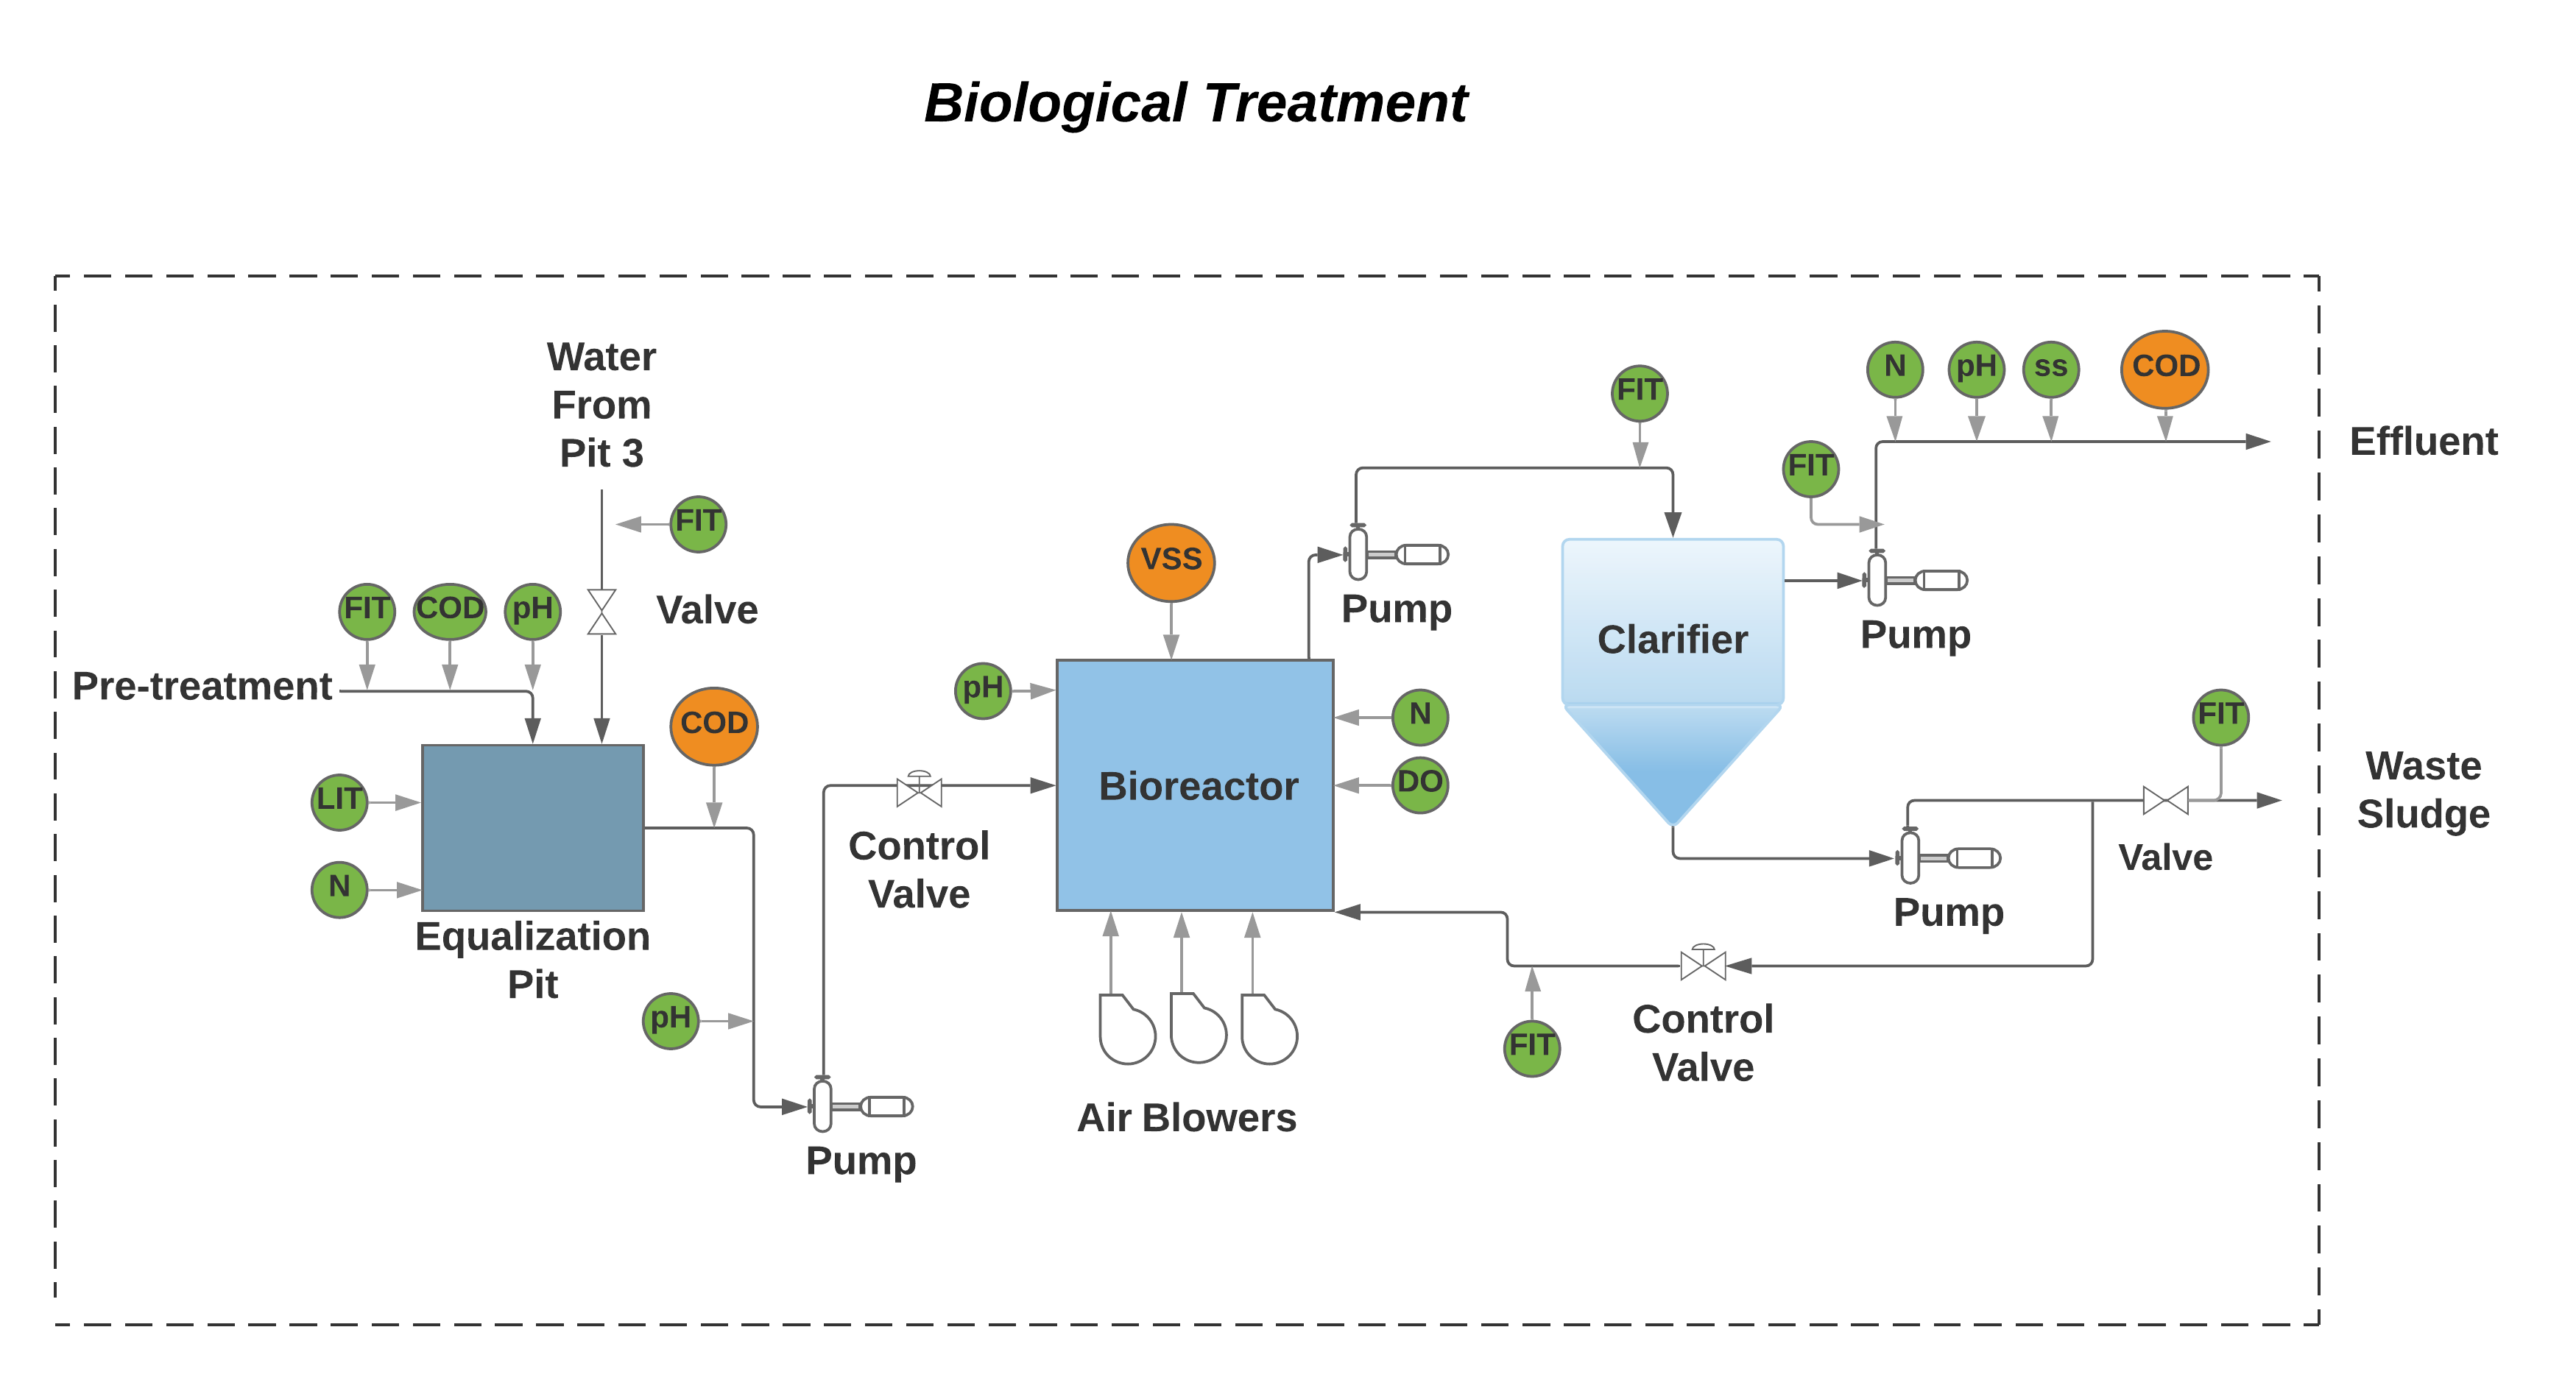
\includegraphics[width=\linewidth]{figures/Ch4/Biological-treatment-stage.png}
\caption{Biological Treatment Stage}
\label{f:Biological-treatment}
\end{figure}

This work uses python programming language to implement the prediction system, supported by several libraries such as Numpy, Pandas, Tensor Flow, Sci-kit Learn, Matplotlib, among others. A GitHub repository contains the files corresponding to code, models, and some results \footnote{\url{https://github.com/carloscp3009/Machine-Learning-Approaches-for-Industrial-data-forecasting}}. The study utilizes 343 data samples from a wastewater treatment facility located in Nantong, China. Measurements correspond to most of the year 2018 and present a daily frequency, which experts consider accurate to capture the process dynamics. The measured variables of the process available for this work are:

\begin{itemize}
 \item	Flow
 \item	COD of influent water
 \item	Suspended solids in influent water (SS)
 \item	Mixed liquor suspended solids (MLSS)
 \item	Mixed liquor volatile suspended solids (MLVSS)
 \item	Nitrogen (N)
 \item	pH
 \item	Mixed liquor dissolved oxygen (DO)
 \item	Food to microorganism (F/M)
\end{itemize}

The following nomenclature determines the stage of the process where the variable is measured.

\begin{itemize}
 \item	EQ = Equalizer
 \item	BIO = Bioreactor
 \item	BT\textsubscript{N}= Bioreactor Pit N
 \item	BT\textsubscript{C}= Bioreactor Pit C
 \item	Clari = Clarifier
 \item	OxT = Oxidation Tank
 \item	D = Discharge Pit
\end{itemize}

The exogenous variables used as inputs of the system are selected using the Pearson correlation. This enhances the model learning capability by reducing the noise of not correlated variables and decreasing the number of trainable parameters which implies a model complexity reduction. Table 1 presents the Person correlation of the three target variables this study cover. 

After variable selection, the dataset is split into training, validation and test sets. However, in this case, the data was split into training and test sets since the number of samples was small in comparison with the amount of data used to train an ANN. It is important to note that a computational technique must be selected. As mentioned before in related works in Table 3, about 64.71\% of the work of authors used an algorithm from the ANN group to develop forecast models. It has been verified that neural networks have suitable results in the area since the water treatment process is characterized by being nonlinear in behavior, so if they are used properly, they can represent the dynamics of this process very well. Once the model was selected, the model was trained and brought into operating condition to estimate COD. An error measure is necessary to support the performance of the model. Therefore, the MAPE), defined as shown in Equation (1), was chosen to quantify the ANN error. In this equation, x\textsubscript{i} represents the actual point, which is intended to be predicted, x\textsubscript{i} represents the predicted values of that observed point and N is the number of observed values that are intended to be predicted.

\section{Approach 1}
\label{s:Approach1}

Figure 5 shows in more detail how the model is conceived and how the COD forecasting is achieved. First, the objective variable taken from the dataset is studied using a time-series decomposition technique that transforms the variable into three additive components: trend, seasonality and residual. Leveraging an auto correlation study over the components, the first two are estimated using their past values. On the other hand, the residual component is estimated using an ANN, which received exogenous variables selected from a correlation study and a past value of the same component. Finally, the addition of the three components provides the COD prediction. 

\begin{figure}[h]
\centering
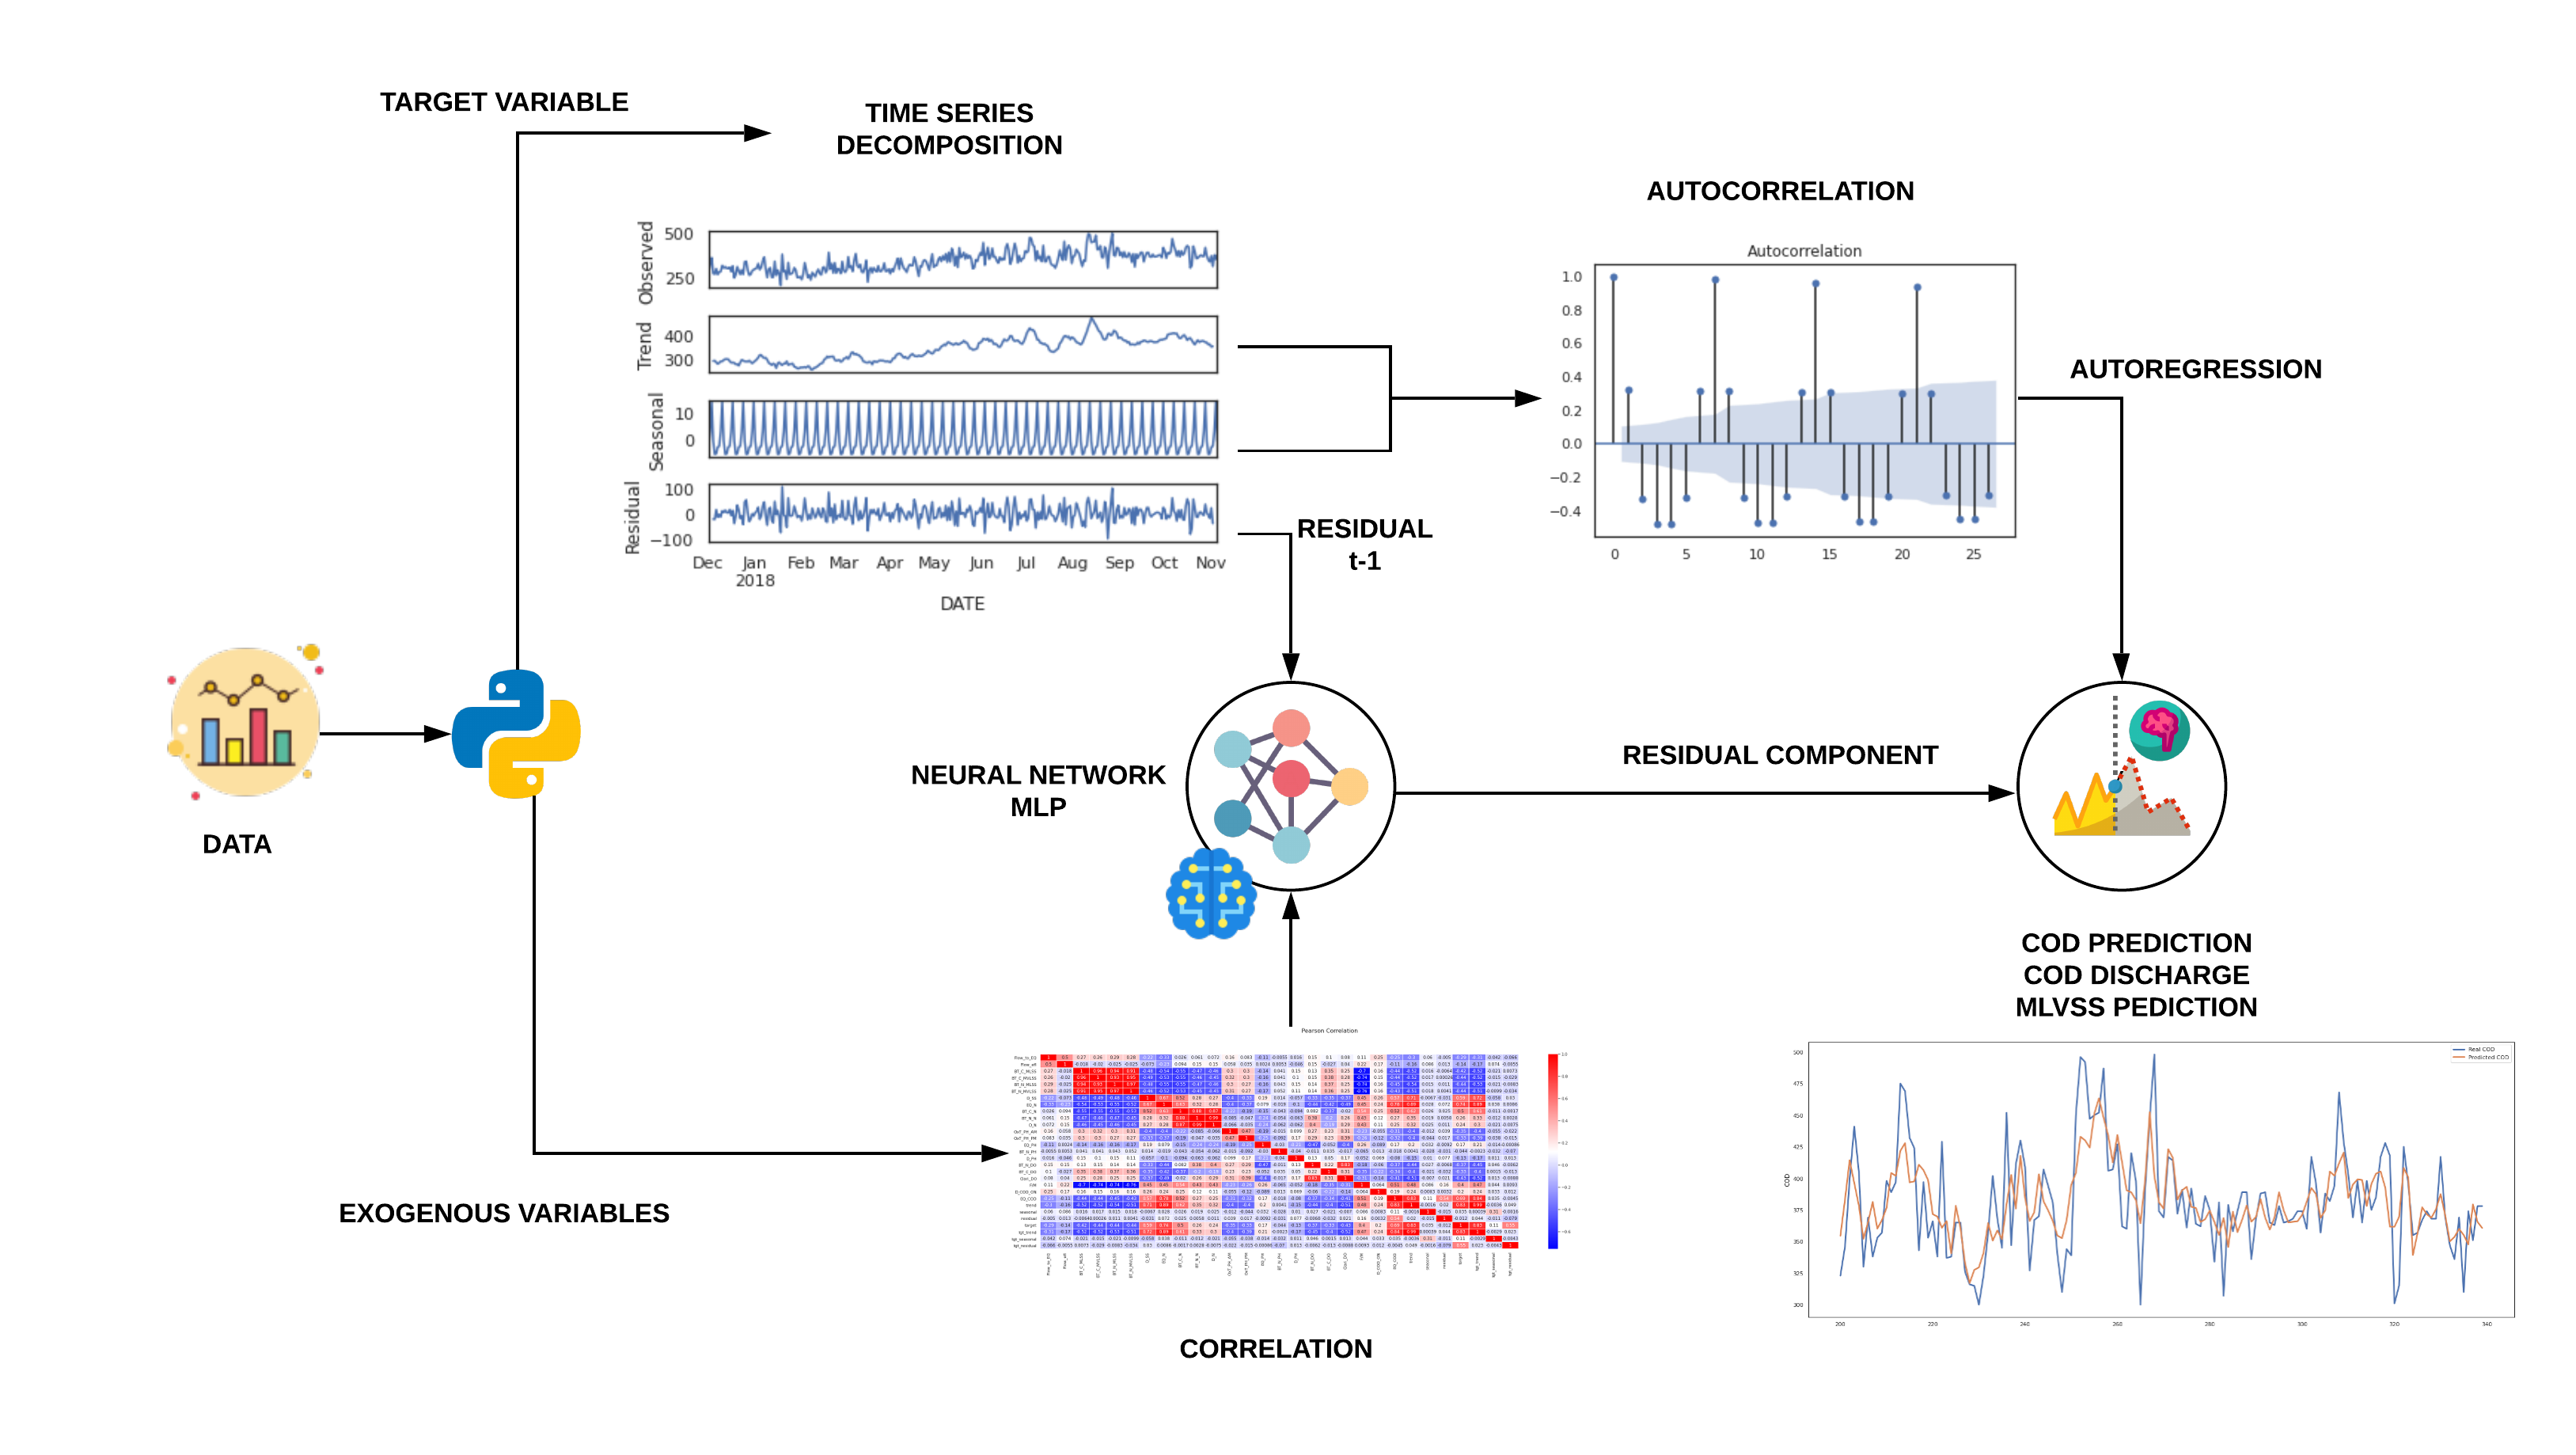
\includegraphics[width=\linewidth]{figures/Ch4/Approach1.png}
\caption{Approach 1}
\label{f:Approach 1}
\end{figure}

\subsection{Time Series Decomposition}
\subsection{Autocorrelation Study}
\subsection{Model Design}

\section{Approach 2}
\label{s:Approach2}

\begin{figure}[h]
\centering
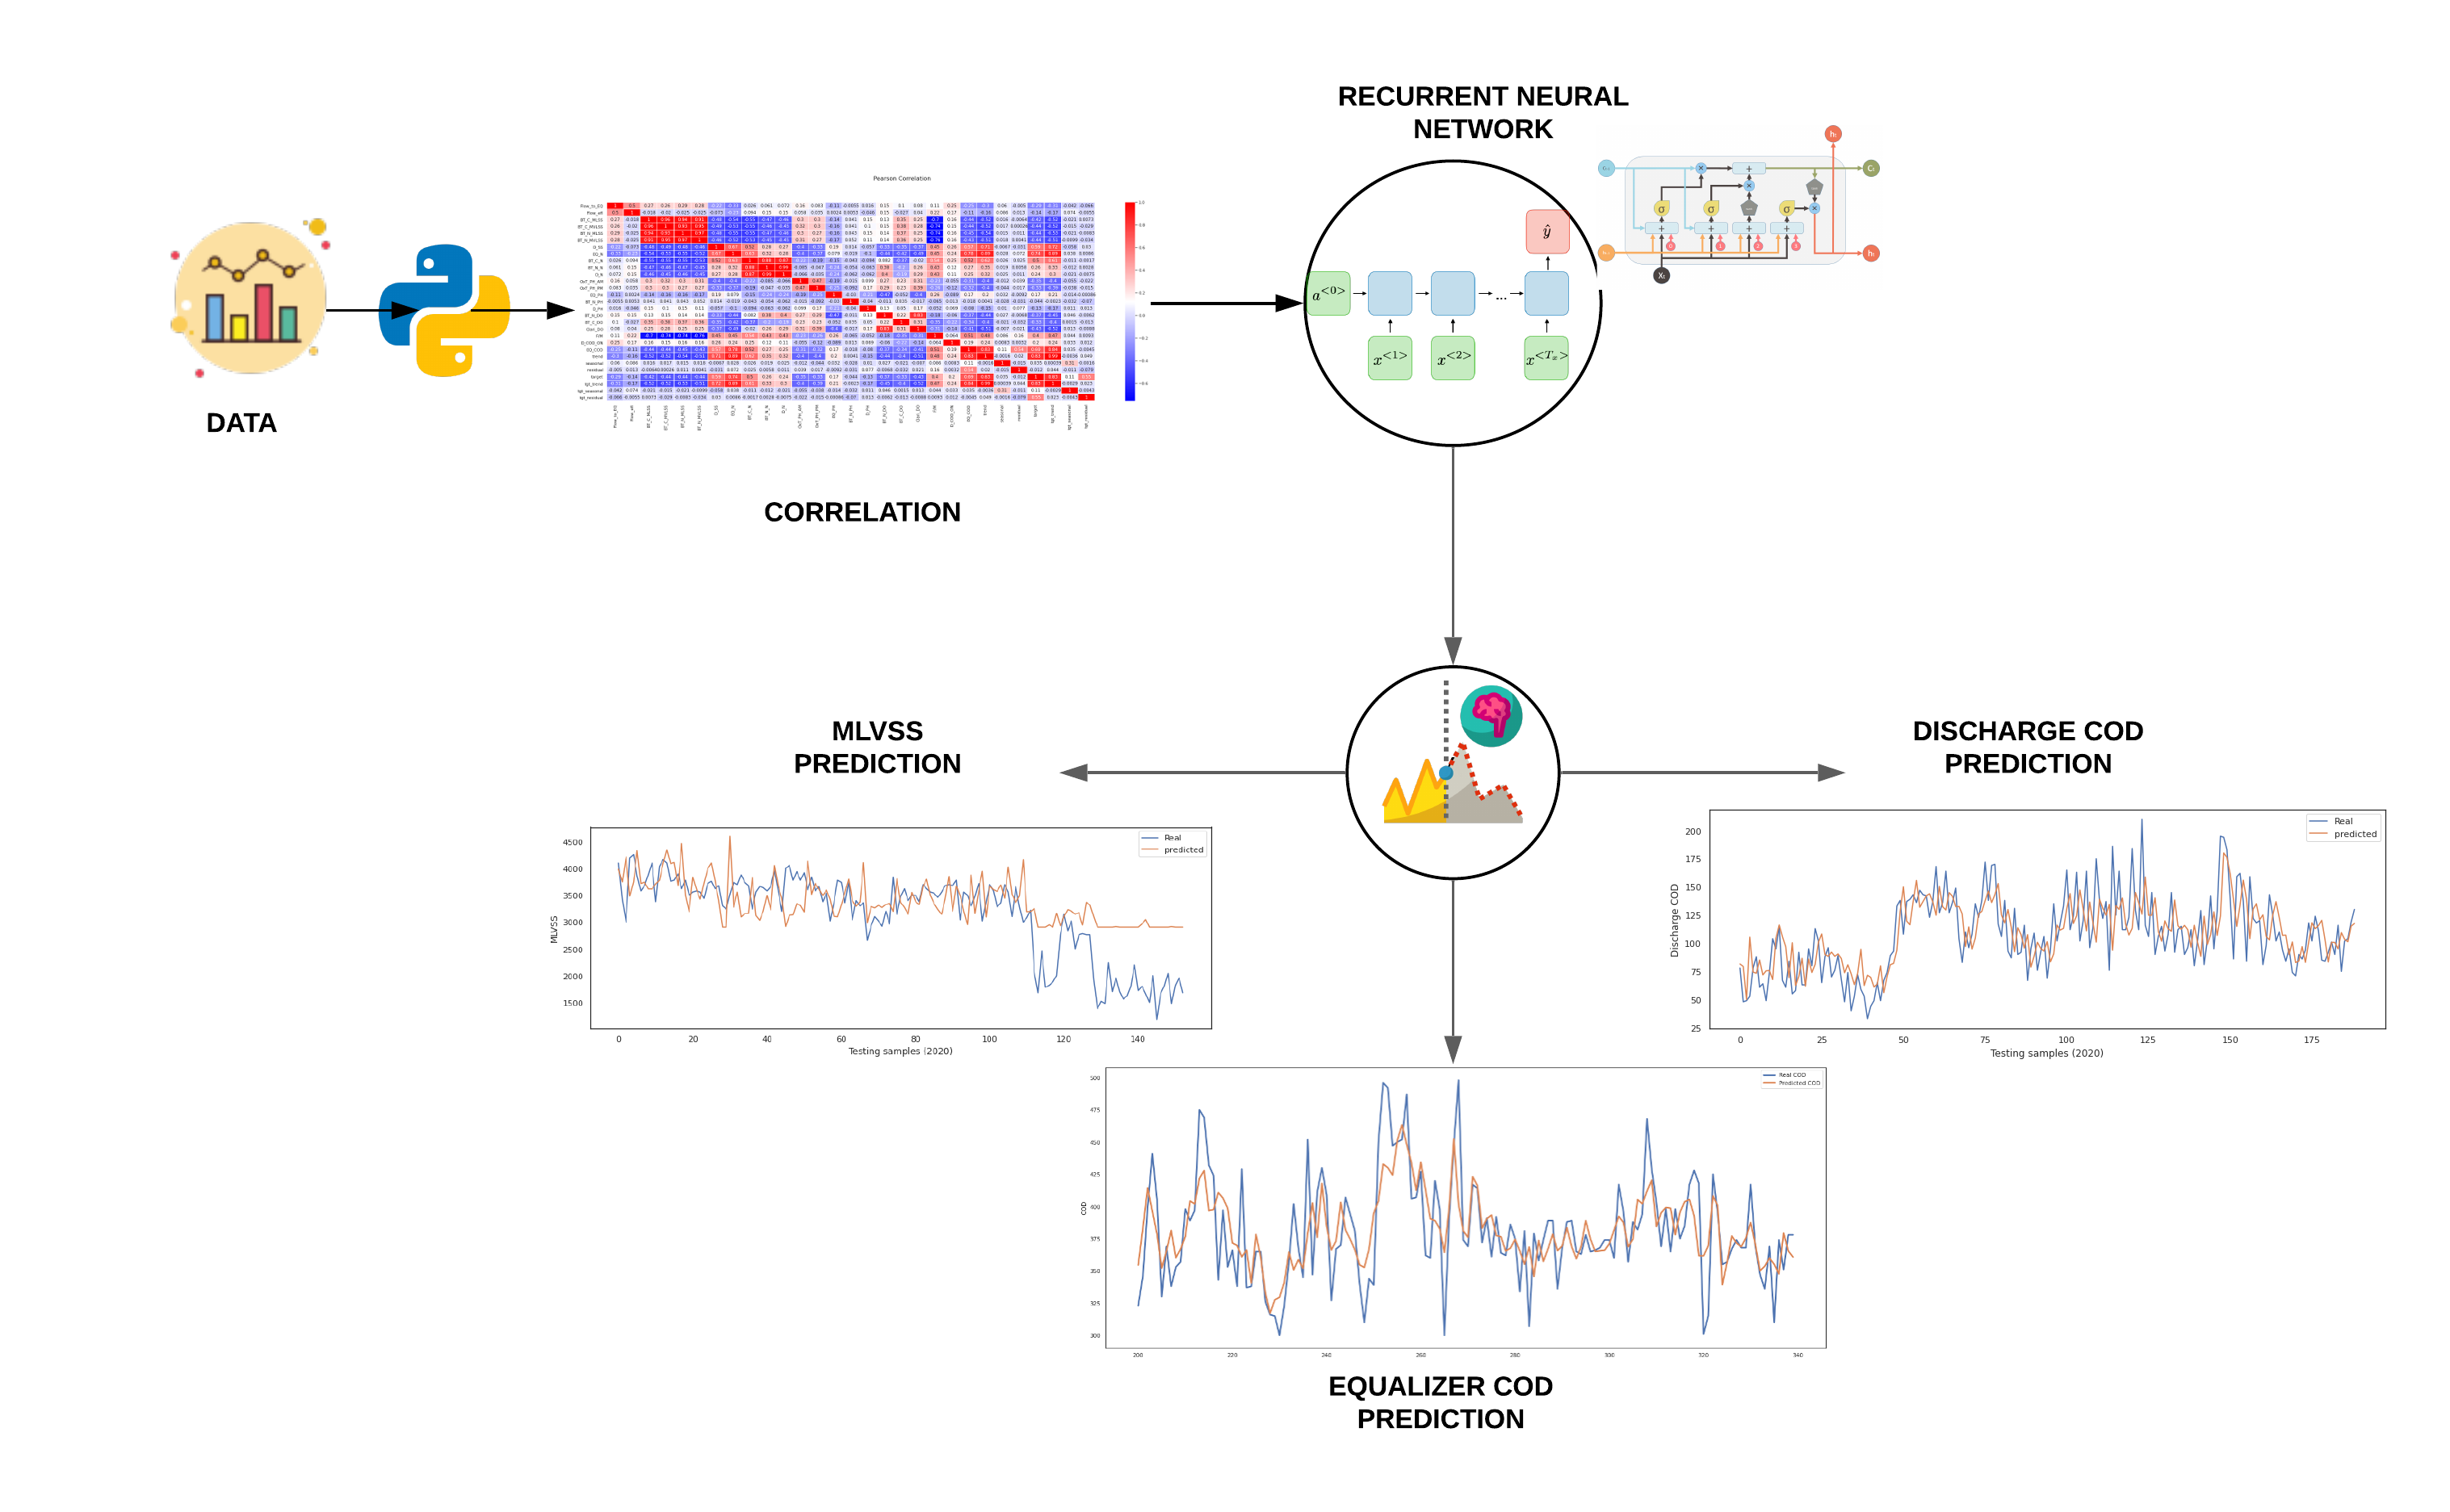
\includegraphics[width=\linewidth]{figures/Ch4/Approach2.png}
\caption{Approach 2}
\label{f:Approach 2}
\end{figure}

\section{Approach 3}
\label{s:Approach3}

\begin{figure}[h]
\centering
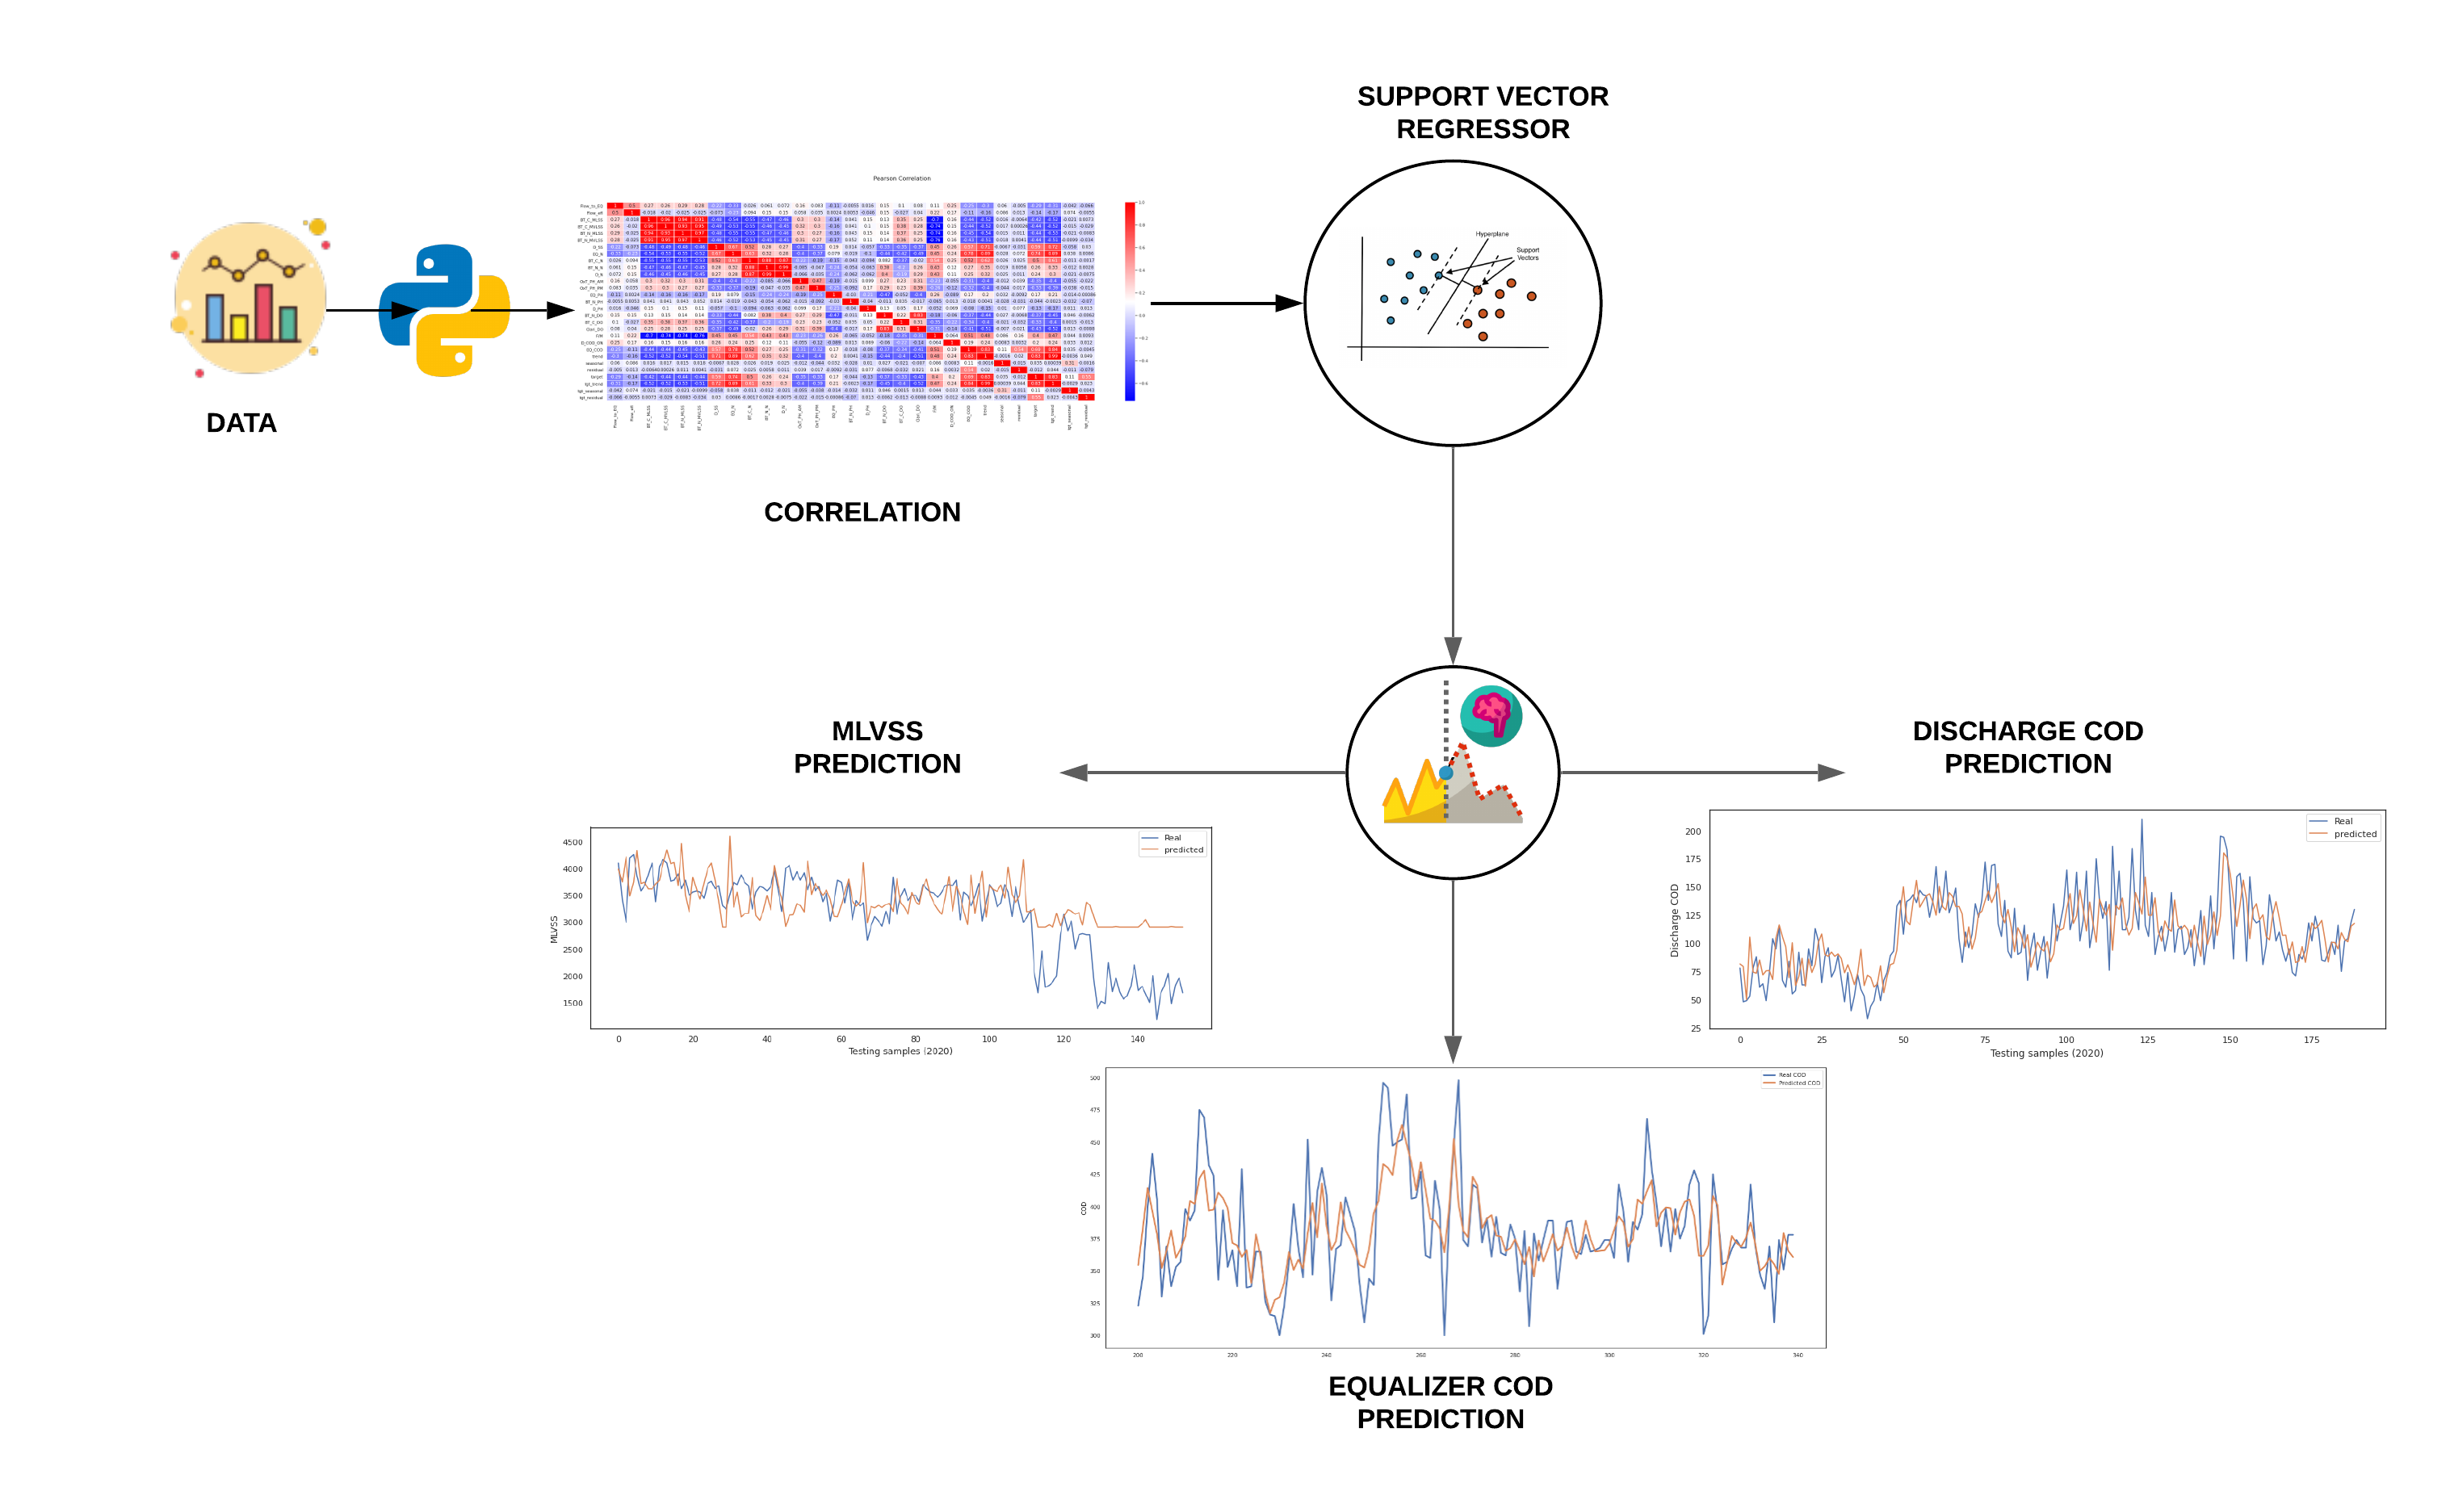
\includegraphics[width=\linewidth]{figures/Ch4/Approach3.png}
\caption{Approach 3}
\label{f:Approach 3}
\end{figure}



\section{Summary}
\label{s:Contribution-1-Summary}

The final section of each major chapter should summarize the chapter. In comparison to the chapter, the summary should be short ($\frac{1}{2}$ to $2$ pages is normal).